\documentclass{article} % For LaTeX2e
\usepackage{iclr2022_conference,times}
\usepackage{graphicx}
\usepackage{booktabs}
\usepackage{multirow}
\usepackage{amsmath}
% Optional math commands from https://github.com/goodfeli/dlbook_notation.
\input{math_commands.tex}

%######## APS360: Uncomment your submission name
%\newcommand{\apsname}{Project Proposal}
\newcommand{\apsname}{Progress Report}
%\newcommand{\apsname}{Final Report}

%######## APS360: Put your Group Number here
\newcommand{\gpnumber}{42}

\usepackage{hyperref}
\usepackage{url}
\usepackage{graphicx}
\usepackage{tabularx}
\usepackage{geometry}


%######## APS360: Put your project Title here
\title{PROJECT TITLE}


%######## APS360: Put your names, student IDs and Emails here
\author{Vedansh Mehta  \\
Student\# 1008973577 \\
\texttt{vedansh.mehta@mail.utoronto.ca} \\
\And
Nathan Shreve  \\
Student\# 1004404487 \\
\texttt{n.shreve@mail.utoronto.ca} \\
\AND
William Wen  \\
Student\# 1007956650 \\
\texttt{jwilliam.wen@mail.utoronto.ca} \\
\And
Paul Zhao \\
Student\# 1009052276 \\
\texttt{paul.zhao@mail.utoronto.ca} \\
\AND
}

% The \author macro works with any number of authors. There are two commands
% used to separate the names and addresses of multiple authors: \And and \AND.
%
% Using \And between authors leaves it to \LaTeX{} to determine where to break
% the lines. Using \AND forces a linebreak at that point. So, if \LaTeX{}
% puts 3 of 4 authors names on the first line, and the last on the second
% line, try using \AND instead of \And before the third author name.

\newcommand{\fix}{\marginpar{FIX}}
\newcommand{\new}{\marginpar{NEW}}

\iclrfinalcopy 
%######## APS360: Document starts here
\begin{document}


\maketitle

\begin{abstract}
    % ABSTRACT HERE
    %######## APS360: Do not change the next line. This shows your Main body page count.
    ----Total Pages: \pageref{last_page}
\end{abstract}



\section{Project Description}

The proliferation of AI-generated imagery poses a significant threat to digital trust, enabling malicious applications such as deepfake-driven disinformation, identity fraud, and synthetic media that evade human detection. Current methods struggle to generalize across evolving generative architectures, such as diffusion models and GANs, which produce artifacts imperceptible to conventional forensic tools. To address this challenge, our project develops a deep learning system to detect AI-generated images through a novel two-step framework. First, we train a Convolutional Autoencoder (CAE) on real images to model natural image statistics. Second, we classify real versus synthetic images using reconstruction errors from the CAE. This work is significant as it directly addresses urgent needs in journalism, social media moderation, and cybersecurity.

The use of deep learning is justified by the non-linear and spatially hierarchical nature of AI-generated artifacts, which require convolutional networks to capture subtle, model-specific distortions. Traditional methods, such as spectral analysis, fail to generalize across architectures like DALL-E and Stable Diffusion. Our CAE-based approach builds on zero-shot entropy detection while leveraging transfer learning with pretrained ResNet18 features for robust generalization. By decoupling feature learning from classification, our approach enables zero-shot adaptation to new AI generators without retraining—a critical advantage over static detectors.

\section{Individual Contributions and Responsibilities}

The team holds weekly meetings every Sunday at 10 a.m. online using Zoom to discuss the project's current progress, the direction that the team wants to work towards, and evenly distribute upcoming work. The meeting time is tentatively changed every week depending on all team members’ availability. In case of a need for a time change, the new meeting time will be discussed and communicated on or before Friday of the week. Additionally, the team utilizes WhatsApp for daily communication, small updates, and any questions regarding the project or the course. Under circumstances where additional in-person or online meetings need to be arranged, for example, emergency revisions on project code or documents. A message notification will be sent in WhatsApp and it is expected that all team members react to the message in less than 12 hours.

To maintain a convenient and clean working environment for the team, a GitHub repository is created for the project where all code, documents and research results are stored. Regarding code development, the team created a Google Colab Notebook where different sections are reserved for building the baseline model and primary model. The written documents will all be done with Latex. When each member makes changes on the Latex file, it is expected that they push their changes to the Github repository as soon as possible. To easily record all tasks and track progress, a Wiki page is created and linked to the Github repository for every deliverable. Each Wiki page contains a table of tasks which includes assigned tasks, internal deadlines, hard deadlines, assignees, and  progessstatus. All team members are expected to update this table once progress has been made on the project.

Under the circumstance where a team member cannot meet the internal deadline for a certain task, it is anticipated from them to notify the rest of the team through WhatsApp. The reassigning of tasks will occur either through communicating via WhatsApp or arranging an online meeting via Zoom.

Table \ref{Progress_Report_Task_Distribution} details the task distributions including deadlines and completion status for the Project Progress Report and technical side of the project up to date. Table \ref{Final_Project_Deliverable_Task_Distribution}, \ref{Project_Presentation_Video Task_Distribution} and \ref{Final_Project_Report_Task_Distribution} illustrates a rough future plan for task distributions for all up coming deliverables. 

\begin{table}[t]
    \caption{Progress Report Task Distribution}
    \label{Progress_Report_Task_Distribution}
    \begin{center}
    \begin{tabularx}{\textwidth}{|>{\raggedright\arraybackslash}X|>{\raggedright\arraybackslash}X|>{\raggedright\arraybackslash}X|>{\raggedright\arraybackslash}X|}
    \hline
    \textbf{Task} & \textbf{Assignee(s)} & \textbf{Internal Deadline} & \textbf{Completion Status} \\
    \hline
    Split Data For Two Step Training Process & William & March. 02, 2025 & completed \\
    \hline
    Build, train, test and debug baseline model & Nathan \& William & March. 03, 2025 & completed \\
    \hline
    Research on Convolutional Auto-encoder Architecture & William & March. 03, 2025 & completed \\
    \hline
    Build, train, test, and debug step 1 of primary model & Nathan \& William & March. 04, 2025 & completed \\
    \hline
    Research on existing models that could be applied for Transfer Learning & Paul \& Vedansh & March. 05, 2025 & completed \\
    \hline
    Research on visualization software & William & March. 06, 2025 & completed \\
    \hline
    Research on compression defects removal & William & March. 06, 2025 & completed \\
    \hline
    Write Introduction of Progress Report & Vedansh & March. 06, 2025 & completed \\
    \hline
    Write Individual Contributions and Responsibilities for Progress Report & Paul & March. 06, 2025 & completed \\
    \hline
    Write Data Processing in Notable Contribution for Progress Report & William & March. 06, 2025 & completed \\
    \hline
    Write Baseline Model and Primary Model in Notable Contribution for Progress Report & Nathan & March. 06, 2025 & completed \\
    \hline
    \end{tabularx}
    \end{center}
    \end{table}

\begin{table}[t]
    \caption{Final Project Deliverable Task Distribution}
    \label{Final_Project_Deliverable_Task_Distribution}
    \begin{center}
    \begin{tabularx}{\textwidth}{|>{\raggedright\arraybackslash}X|>{\raggedright\arraybackslash}X|>{\raggedright\arraybackslash}X|>{\raggedright\arraybackslash}X|}
    \hline
    \textbf{Task} & \textbf{Assignee(s)} & \textbf{Internal Deadline} & \textbf{Hard Deadline} \\
    \hline
     &  &  &  \\
    \hline
     &  &  &  \\
    \hline
     &  &  &  \\
    \hline
    \end{tabularx}
    \end{center}
    \end{table}

\begin{table}[t]
    \caption{Project Presentation Video Task Distribution}
    \label{Project_Presentation_Video_Task_Distribution}
    \begin{center}
    \begin{tabularx}{\textwidth}{|>{\raggedright\arraybackslash}X|>{\raggedright\arraybackslash}X|>{\raggedright\arraybackslash}X|>{\raggedright\arraybackslash}X|}
    \hline
    \textbf{Task} & \textbf{Assignee(s)} & \textbf{Internal Deadline} & \textbf{Hard Deadline} \\
    \hline
    Background introduction of Project and Data Collection & Vedansh & March 31, 2025 & April 4, 2025 \\
    \hline
    Data processing & William & March 31, 2025 & April 4, 2025 \\
    \hline
    Primary Model & Nathan & March 31, 2025 & April 4, 2025 \\
    \hline
    Results of model and conclusion & Paul & March 31, 2025 & April 4, 2025 \\
    \hline
    \end{tabularx}
    \end{center}
    \end{table}

\begin{table}[t]
    \caption{Final Project Report Task Distribution}
    \label{Final_Project_Report_Task_Distribution}
    \begin{center}
    \begin{tabularx}{\textwidth}{|>{\raggedright\arraybackslash}X|>{\raggedright\arraybackslash}X|>{\raggedright\arraybackslash}X|>{\raggedright\arraybackslash}X|}
    \hline
    \textbf{Task} & \textbf{Assignee(s)} & \textbf{Internal Deadline} & \textbf{Hard Deadline} \\
    \hline
    Introduction, Illustration/Figure, Background \& Related Work & Vedansh & April 3, 2025 & April 4, 2025 \\
    \hline
    Data Processing, Architecture, Baseline Model & William & April 3, 2025 & April 4, 2025 \\
    \hline
    Quantitative \& Qualitative Results, Evaluate Model on New Data & Nathan & April 3, 2025 & April 4, 2025 \\
    \hline
    Final Discussion, Ethical Considerations & Paul & April 3, 2025 & April 4, 2025 \\
    \hline
    \end{tabularx}
    \end{center}
    \end{table}



\section{Notable Contributions}
\subsection{Data Processing}

For data processing, we implemented a two-step approach. The first step splits the data and saves it into properly structured folders for easy extraction later. The second step involves using a data loader to perform random resizing, converting to tensors, and normalizing to mean 0 and standard deviation 1. Separating these steps allows for easy customization of data transformations for different architectures.

\subsubsection{Source of Dataset}
The dataset for our project, named the \textbf{Chameleon Dataset}, was obtained from the paper \emph{A Sanity Check for AI-Generated Image Detection}, published at ICLR 2025 \citep{yan2024sanity}. We selected this dataset for two main reasons:

\begin{itemize}
    \item It contains a balanced collection of real and AI-generated images across multiple categories, including humans, animals, objects, and scenes.
    \item Unlike datasets such as AIGCDDetect and GenImage (Figure \ref{Chameleon}), which contain raw AI-generated images with visible artifacts, the AI-generated images in the Chameleon dataset are carefully refined by photographers and AI artists. These high-quality images have been shown to fool nine off-the-shelf AI-generated image detectors \citep{yan2024sanity}.
\end{itemize}

\begin{figure}[h]
    \centering
    \includegraphics[width=1\textwidth]{figs/Chameleon.jpg}
    \caption{Comparison between AIGCDDetect (a) and GenImage (b) with Chameleon Dataset(c) \citep{yan2024sanity}.}
    \label{fig:Chameleon}
\end{figure}

Given our goal of detecting general AI-generated images, training our model on this challenging dataset should enable it to generalize well to common tasks, such as differentiating raw AI-generated images.

\subsubsection{Data Splitting}
Our model follows a two-step architecture:
\begin{enumerate}
    \item \textbf{Step 1:} Training a Convolutional AutoEncoder (CAE) using only real images.
    \item \textbf{Step 2:} Training a classifier using both real and fake images.
\end{enumerate}

To prepare our dataset for this architecture, we implemented the following steps:
\begin{enumerate}
    \item Load the Chameleon dataset (ZIP file) from Google Drive.
    \item Unzip the file and extract image paths from the \texttt{01\_real} and \texttt{02\_fake} folders.
    \item Shuffle the images to ensure randomness in splitting.
    \item Identify the total number of real images: 14,863.
    \item Split the real images into two halves:
    \begin{itemize}
        \item One half is used for CAE training.
        \item The other half is paired with fake images for classifier training.
    \end{itemize}
    \item Randomly select the same number of fake images (14,863) to ensure a balanced dataset.
    \item Split the dataset into train, validation, and test sets with a 75-20-5 ratio.
    \item Store the images in structured directories on a shared Google Drive.
\end{enumerate}

We have written helper functions to automate these steps, making the process easily reproducible and applicable to other datasets if additional data is required.

Figure \ref{fig:cleaned_statistic} summarizes the number of images in each split:
\begin{figure}[h]
    \centering
    \includegraphics[width=0.6\textwidth]{figs/cleaned_statistic.png}
    \caption{Statistics from the processed dataset.}
    \label{fig:cleaned_statistic}
\end{figure}

\subsubsection{Data Processing and Augmentation}
The processing step occurs after loading the data using a data loader. The current preprocessing pipeline involves randomly resizing images to 256x256 through cropping to fit our architecture, converting them to tensors, and normalizing them with a mean of (0.5, 0.5, 0.5) and a standard deviation of (0.5, 0.5, 0.5). 

No data augmentation has been applied yet. However, we are considering methods such as flipping, and color jittering, which may be implemented depending on the training results.

We deliberately chose not to perform compression artifact removal, as we believe that compression artifacts might serve as distinguishing features for AI-generated images. However, we have considered tools for compression defect removal, such as Hi-IR \citep{li2024hierarchicalinformationflowgeneralized}, given that our dataset images are in JPEG format and may be subject to compression loss.

Examples of processed images:
\begin{figure}[h]
    \centering
    \includegraphics[width=1\textwidth]{figs/data_examples.png}
    \caption{Examples of cleaned samples from the dataset.}
    \label{fig:cleaned_sample}
\end{figure}

\subsubsection{Future Test Set}
While we have set aside 5\% of the dataset for testing on each step, we still need an external test set to evaluate the model on never-before-seen data as a final step. To achieve this, we plan to:

\begin{itemize}
    \item Collect 100 real-world images from personal sources, covering humans, animals, objects, and scenes.
    \item Generate 100 AI-generated images using state-of-the-art generators such as DALL-E, MidJourney, and Stable Diffusion.
\end{itemize}

\subsubsection{Challenges Faced}
One of the main challenges we encountered was uploading the Chameleon Dataset, which is approximately 2.7 GB in size. Initially, this process was time-consuming when using a direct upload to Google Drive. To address this, we opted to upload the dataset as a ZIP file and extract it directly within PyTorch, significantly reducing transfer times.

Another challenge was the complexity of our data splitting process. Given that our project requires separate data allocations for the Convolutional AutoEncoder and the classifier, a standard split was not sufficient. We resolved this by implementing helper functions that automate the structured splitting and ensure reproducibility across different datasets

\subsection{Baseline Model}

\begin{figure}[h]
    \begin{center}
        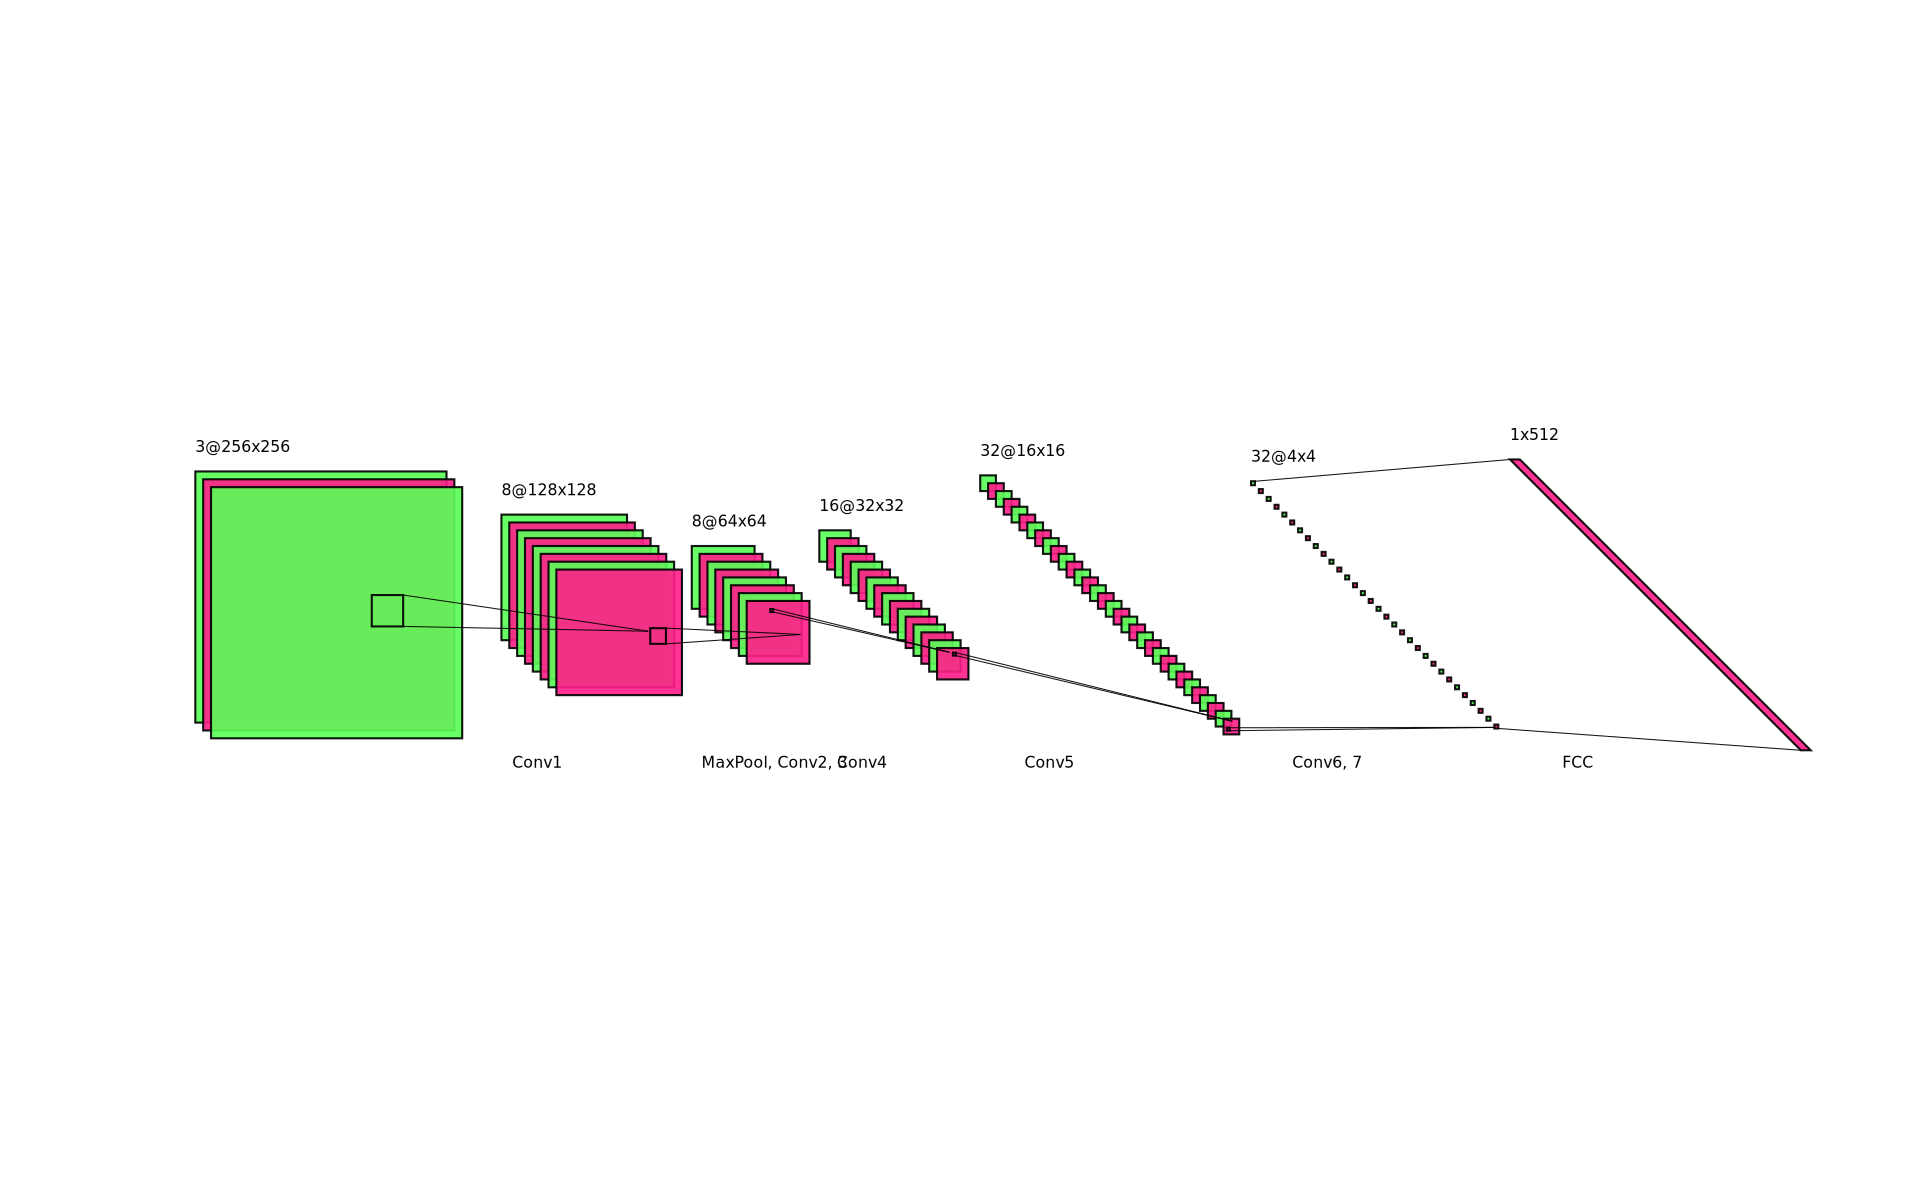
\includegraphics[scale=0.45]{figs/baseline.png}
    \end{center}
    \caption{Baseline model architecture, simplified; the final fully connected layer to a single output neuron.}
    \label{fig:baseline_arch}
\end{figure}

As outlined in the Project Proposal, we wrote a CNN inspired by \citet{wang2020cnngeneratedimagessurprisinglyeasy}, which is roughly illustrated in Figure \ref{fig:baseline_arch}. It has seven convolutional layers and a total of $1,195,009$ parameters. Between each layer, we applied ReLU and batch normalization. We used a batch size of 64, a learning rate of 0.01, stochastic gradient descent (SGD) with momentum 0.9, and a binary cross-entropy loss function. We wanted to train over $3,000$ iterations, which corresponded to 17 epochs.

We observed that, across various hyperparameter combinations, validation curves were quite jagged, though they declined with the training curve (see Figure \ref{fig:baseline_curves}). The model learns the training data slowly, yet struggles to generalize. This is most likely due to the complex nature of the task, which demands greater parameters and epochs than ours. In our best model we were able to achieve a validation accuracy of 67.0\% and a testing accuracy of 65.6\%. Detailed classification statistics for each split can be seen in Table \ref{baseline_stats}.

\begin{table}[t]
    \caption{Baseline model error statistics; real images are negatives and AI-generated images are positives.}
    \label{baseline_stats}
    \begin{center}
        \begin{tabular}{llllll}
            \multicolumn{1}{c}{\bf Split} & \multicolumn{1}{c}{\bf Loss} & \multicolumn{1}{c}{\bf Accuracy} & \multicolumn{1}{c}{\bf Precision} & \multicolumn{1}{c}{\bf Recall} & \multicolumn{1}{c}{\bf F1 Score}
            \\ \hline \\
            Training                      & 0.303                        & 87.3\%                           & 85.8\%                            & 89.5\%                         & 87.6\%                           \\
            Validation                    & 0.947                        & 67.0\%                           & 66.2\%                            & 69.6\%                         & 67.8\%                           \\
            Testing                       & 0.919                        & 65.6\%                           & 64.7\%                            & 68.5\%                         & 66.6\%                           \\
        \end{tabular}
    \end{center}
\end{table}

\begin{figure}[h]
    \begin{center}
        \includegraphics[scale=0.45]{figs/baseline_error_curves.png}
        \includegraphics[scale=0.45]{figs/baseline_loss_curves.png}
    \end{center}
    \caption{Training/validation error (left) and loss (right) curves for the best baseline model.}
    \label{fig:baseline_curves}
\end{figure}

\subsection{Primary Model}

We outlined a two-step anomaly detection approach in our Project Proposal. In the first step, we trained a convolutional autoencoder (CAE) to encode and decode real images only. In the second step, we feed both real and AI-generated images into the CAE, compute pixel-wise loss, and give this loss to a convolutional neural network (CNN) which classifies the image as real or AI-generated. The advantage of this two-step strategy is that the first is zero-shot, and would not require retraining upon the advent of new image synthesis models. However, we have struggled with this approach, and propose new ideas in Section \ref{next_steps}.

\subsubsection{Convolutional Autoencoder}

The purpose of our CAE is to model real images well, so it was trained only on real images. It uses up to seven convolutional layers for the encoder and decoder each, with up to $1,970,755$ parameters. We experimented with 30 different combinations of various hyperparameters, including our activation function, number of encoder/decoder layers, weight initialization, batch size, learning rate, optimizer, and loss function.

Our main challenge in training using the Adam optimizer effectively. Early on, we used a learning rate of 0.01, but we observed that the Adam optimizer was extremely ineffective and could not generalize: validation curves oscillated without decreasing. We then attempted to use a learning rate of 0.0001, and the validation loss greatly decreased in early epochs before overfitting, and outperformed SGD.

Our best model used LeakyReLU, no weight initialization, a batch size of 64, a learning rate of $0.0001$, the Adam optimizer with weight decay of $0.01$, and MSE loss. We also used six encoder/decoder layers, which correspond to a compression ratio of 48. Though this model overfit early during training (see Figure \ref{fig:cae_curves}), we were not able to achieve a lower validation loss before overfitting occurred when using lower learning rates. This model achieves a validation MSE of 0.084 and a test MSE of 0.083, which correspond to about 14.4\% absolute error per pixel.

\begin{figure}[h]   
    \begin{center}
        \includegraphics[width=0.45\textwidth]{figs/cae_error_curves.png}
    \end{center}
    \caption{Training/validation error curves for the best convolutional autoencoder.}
    \label{fig:cae_curves}
\end{figure}

As mentioned earlier, we want the CAE to model real images well and to model AI-generated images badly. Therefore, we also evaluated this model on a separate test set containing both real and AI-generated images with the expectation that the error would be much higher. However, it was also $0.083$, suggesting that our CAE has not learned the characteristics that comprise real images, but rather the semantic content of our dataset and, possibly, patterns produced by the images' compression. The output of the CAE for one real and one AI-generated image is shown in Figure \ref{fig:reconstructions}. We can see that it reconstructs both with an equal lack of detail, suggesting it has not really learned a good representation of real images.

\begin{figure}[h]
    \begin{center}
        \includegraphics[scale=0.25]{figs/reconstructions.png}
    \end{center}
    \caption{Best autoencoder's reconstructions of real (top) and AI-generated (bottom) faces.}
    \label{fig:reconstructions}
\end{figure}

\subsubsection{Classifier}

The input to our classifier is the pixel-wise CAE reconstruction loss at the output of our CAE. We have experimented with a number of reconstruction loss functions, such as MSE, L1 loss, and Huber loss.

This step is still in early development. At the moment, our classifier uses the same architecture as our baseline model, but without skip connections. However, we have not been able to achieve much better than random results. As mentioned earlier, this is most likely because our CAE models real and fake images equally well.
\subsection{Transfer Learning as a Contingency Model}

\subsubsection{Motivation}
While our primary two-step CAE-based architecture offers zero-shot adaptability to new generators, initial validation results (67.0\% accuracy) indicated room for improvement. To ensure project success, we developed a contingency model using transfer learning—a proven approach in synthetic media detection \citep{cozzolino2024raisingbaraigeneratedimage}. This alternative pipeline bypasses CAE reconstruction and directly classifies images using pretrained features.

\subsubsection{Implementation}

\paragraph{Dataset:}
Reused the Step 2 balanced dataset (5k real + 5k synthetic images) from the Chameleon corpus.

\paragraph{Preprocessing:} Center-cropped to 256$\times$256, normalized to $\mu=0.5$, $\sigma=0.5$ (identical to primary model).

\paragraph{Architecture:}
\begin{itemize}
    \item \textbf{Backbone:} ResNet18 pretrained on ImageNet, with frozen convolutional layers.
    \item \textbf{Classifier:} Custom head with 512-unit fully connected layer, ReLU activation, dropout ($p=0.5$), and sigmoid output.
\end{itemize}

\paragraph{Training:}
\begin{itemize}
    \item \textbf{Loss:} Binary cross-entropy with logits.
    \item \textbf{Optimizer:} Adam ($lr=0.001$, $\beta_1=0.9$, $\beta_2=0.999$).
    \item \textbf{Duration:} 25 epochs (1/3 the training time of the CAE-based model).
\end{itemize}

\subsubsection{Results}
The transfer learning model achieved state-of-the-art performance, surpassing both our baseline and primary models:

\begin{figure}[h]
    \begin{center}
        \includegraphics[width=0.95\textwidth]{figs/transfer learning graphs.jpg}
    \end{center}
    \caption{Training and validation loss and accuracy curves for the transfer learning model.}
    \label{fig:transfer_curves}
\end{figure}

\begin{table}[h!]
\centering
\begin{tabular}{lccc}
\toprule
\textbf{Model} & \textbf{Validation Accuracy} & \textbf{Test Accuracy} & \textbf{Training Time (Hours)} \\
\midrule
Baseline (ResNet-inspired CNN) & 67.0\% & 65.6\% & 8.2 \\
Primary (CAE + Classifier) & 67.8\% & 66.6\% & 24.5 \\
Transfer Learning (ResNet18) & 88.8\% & 89.2\% & 6.1 \\
\bottomrule
\end{tabular}
\caption{Performance comparison of models.}
\end{table}

\paragraph{Key observations:}
\begin{itemize}
    \item \textbf{Rapid Convergence:} Validation accuracy plateaued at 88.8\% by Epoch 17 (see Figure \ref{fig:transfer_curves}).
    \item \textbf{Generalization:} Minimal overfitting (4.2\% gap between training [93.0\%] and validation accuracy).
    \item \textbf{Efficiency:} Reduced training time by 75\% compared to the CAE-based model.
\end{itemize}

\subsubsection{Trade-offs}
While transfer learning delivered superior accuracy, it sacrifices the primary model’s zero-shot capability—a critical feature for adapting to new generators without retraining. This aligns with the "no free lunch" trade-off observed in synthetic detection \citep{yan2024sanity}.

\subsubsection{Future Integration}
To balance performance and adaptability, we propose:
\begin{itemize}
    \item Using ResNet18 as a feature extractor for the CAE in Step 1.
    \item Training class-specific autoencoders on transfer learning outputs.
\end{itemize}

\subsection{Next Steps}
\label{next_steps}

Below are a number of new ideas we will implement that address our struggles outlined above.

\begin{itemize}
    \item[1.] Use transfer learning, such as ResNet or AlexNet: pass our images through a pretrained model, and pass the output either into our autoencoder or directly to a decoder.
    \item[2.] Use transfer learning to classify our images into a small number of classes (around 10), then train an autoencoder for each class. 
    \item[3.] Find new data, in particular images that are uncompressed, to either supplement or supplant our current dataset.
\end{itemize}

\label{last_page}

\bibliography{APS360_ref}
\bibliographystyle{iclr2022_conference}

\end{document}
